% The setting of the project is described based on the scientific literature in a balanced and comprehensive way. The content and relevance of the included literature is understood
\chapter[Background]{Background}
\label{cha:backgr}
This chapter will go over the background of this project, which will cover basic operating system fundamentals, a brief overview of the RISC-V architecture, and the specifics of the board that will be used, which is the Sifive Hifive1 RevB. By the end of the chapter, the reader should be able to understand how parts of the operating system should function, and be able to understand the RISC-V architecture in comparison to the ARM architecture.
\section{Operating System Fundamentals}
An operating system's purpose is to provide an interface between user code and the hardware, such as memory and \ac{io}, to allow the user code to function seamlessly, and allow interaction with users. This has been split into three key sections, as listed by the aims of the project, as process management, memory management and \ac{io} management\cite{modern_operating}.
\subsection{Process Management}
A process is a section of executing code along with the registers that executing code uses. The goal of the operating system is to allow multiple processes to run at once. In a system with multiple cores, this would be possible to do explicitly, as the different cores could simply execute the processes. However the desired number of processes is almost always higher than the number of available cores, and in the world of microprocessors there is rarely more than one cores, so instead processes must be run individually and interleaved to give the illusion of multitasking, provided that this is done at a high enough frequency. There are several methods and approaches to this task\cite{modern_operating}.
\subsubsection{Scheduling Algorithms}
The main approaches to be considered for scheduling algorithms for this project will be a batch approach and an interactive approach. The most important distinction between the two is the inclusion of preemption. In a batch system, a non-preemptive approach will be taken, where once a processes execution is begun, it will be allowed to complete before any other process runs. This creates a simple system and is used is situations where completion of tasks is not expected to be quick. The main challenges of this approach is in process execution time estimation, as this allows the scheduler to order the execution of processes in a way that ensure small tasks are allowed to run. In an interactive system, it is expected from the user that interactions should have quick responses. This introduces the need for preemption, where a processes' execution may be paused after a short period to allow other processes to run. By running each process in small interleaved time slices this allows multiple processes functionally at the same time, which means processes from which a user is expecting a response will not halt other processes\cite{modern_operating}.
\subsection{Memory Management}
The goal of memory management is to streamline how a process can use memory, while at the same time protecting critical sections of memory from faulty or malicious user code. In a system with multiple processes being executed and no memory abstraction, there exists the possibility that two processes attempt to use the same section of memory, creating a conflict that would cause both processes to run incorrectly. This occurs as different processes cannot be aware of each other, and have no choice but to use memory without knowledge of which sections are in use. This can be solved using memory abstraction. The simplest method of this is using address spaces, where each process is given permission to access only segments of directly addressed memory. This prevents each process modifying other processes' memory, and allows each process to behave individually, as long as it is provided with the location of its address space\cite{modern_operating}.
\subsection{IO Management}
The device that the project features will have severely limited \ac{io}. For the purpose of this project there will be two categories of \ac{io}, programmed \ac{io} and interrupt driven \ac{io}. 
\subsubsection{Serial \ac{io}}
Programmable \ac{io} is where actions that require \ac{io} are done in sequence, which will generally function by the user code making an environment call, which will then perform the \ac{io} operation, and return control to the user code once the operation is complete. This is not always desirable, as the operations are often slow and often include polling, which is the process of performing busy operations until a resource is free. During this time all processes are effectively blocked as the the environment call is not being preempted, so this process can significantly slow execution if the data transfer is slow. However this type of \ac{io} can be useful in cases where only small amounts of data is being transferred, for instance in cases where only single bytes are transferred the overhead needed for interrupt driven \ac{io} would be larger than the time lost to busy waiting.
\subsubsection{Interrupt driven \ac{io}}
To avoid the blocking caused by polling, \ac{io} can be interacted with through the use of interrupts. This would be done by a process making an environment call similar to programmable \ac{io}, however in this case only the caller process would be blocked until the \ac{io} operation was complete. It would also enable some form of interrupt, which signals when the \ac{io} function is available to be used. At that point an interrupt will be raised and part of the operation with be completed until the \ac{io} is busy again, at which point execution is returned to all the unblocked processes. This means that there is no time wasted polling, although does introduce overhead in the form of interrupt calls, which if done too often could slow down execution to a similar level as polling.
\section{RISC-V}
RISC-V is a \ac{risc} \ac{isa}, featuring the goal to be completely open. The ISA uses a base integer ISA which can be used on its own or with a number of optional standard extensions, which is part of a goal to avoid `over-architecting' for particular micro-architectures. There are variants for both 32~bit systems and 64 bit systems however for this project only the 32~bit system will be considered\cite{riscv_unpriv}.
\subsection{Base ISA}
The base ISA, known as RV32I, specifies the set of instructions that all RISC-V systems implement, which includes both privileged and unprivileged instructions. The load and store operations allow loading and storing one register to or from memory. This registers can be treated as a word, half word or as a byte. There are the standard arithmetic, logic and shift operations, however immediate values are limited to 12 bits, so operations such as LUI (load upper immediate) may be used to load larger immediate values into a register.\\
Unlike ARM, the RISC-V ISA does not use flags to determine conditional operations. Instead the condition that is used to determine whether a branch is taken or not is included in the branch operation itself, with instructions like BEQ (branch if equal) or BGT (branch if greater than). These are accompanied by comparison operations, which evaluate similar conditions, and produce either a 1 or a 0 in the target register. JAL (jump and link) branches to a specified location while storing a return address, which allows the implementation of subroutines and functions\cite{riscv_unpriv}.
\subsubsection{Privilege levels}
In most systems, there will be some mechanism for differentiating between system level and user level code. This is to prevent user level code from modifying critical sections of the system which would cause unpredictable behaviour, and to maintain security between different parts of user code. In RISC-V, this is implemented through the differentiation between the unprivileged architecture and the privileged architecture and the access to each being controlled by a current privilege mode. RISC-V provides the specification for a number of different modes, the modes that are relevant are the user mode and the machine mode. These modes can be likened to the concept of a normal user and a `super' user, where the super user is allowed to perform actions the normal user cannot. This means a program in user mode can only execute instructions that are from the unprivileged architecture, and can only access memory that is specified by the memory protection. A program in machine mode can use all instructions from both the unprivileged and privileged architecture, and has access to the full memory space.
\subsubsection{Optional Extensions}
% Include info on A, M, and C
There are several optional extensions that can be implemented. This includes the `C' extensions, which includes a reduced number of instructions from the base ISA, but in a 16 bit compressed format. The `M' extension includes 32~bit instructions to perform multiplication and division, as well as a remainder operation. The `A' extension includes a number of atomic memory operations, such as store conditional, swap instructions and memory operations that perform logic operations atomically.
\subsection{Registers}
The registers in RISC-V can be put into two categories, the general purpose registers, and the control and status registers. These are then used on two levels, the programmers level and the system level.
\subsubsection{Programmer Level}
\begin{figure}
    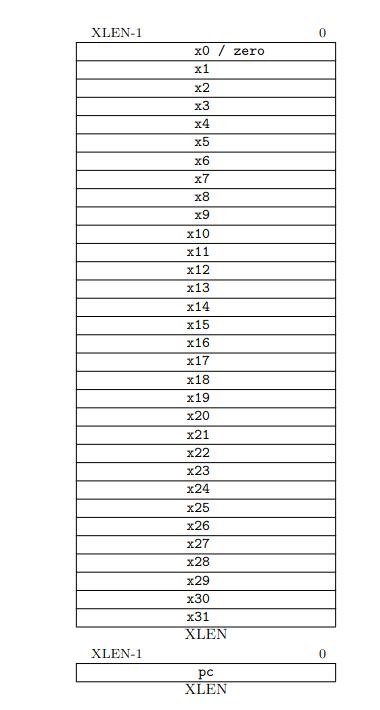
\includegraphics[height=0.6\textheight]{figures/regs.png}
    \centering
    \caption[RISC-V Registers]{This figure shows the registers used at the programmer level, which includes the zero register, 31 general use registers and a program counter, taken from the RISC-V unprivileged architecture\cite{riscv_unpriv}}
\end{figure}
In RISC-V, there are always 32 general purpose registers, x0 to x31. The specific implementation of RISC-V can alter the width (number of bits) of each of the registers; I will be using the rv32i architecture which indicates that each register is 32 bits wide. Each register may be used as the programmer wishes except for x0 which has its value hardwired to zero to facilitate the comparison instructions and allow instructions to not store their output. In addition to the general purpose registers each program also makes use of the \ac{pc}. This stores the address of the current instruction and to the programmer can only read the value stored using the AUIPC (add upper immediate to pc) instruction, and can only be modified through either branch or jump instructions. The pc is an example of one of the  \ac{csrs} that are available to be used by the programmer. Other \ac{csrs} that may be available are the cycle, time and retired instruction CSRs, which display various data about the system; these are accessed through the RD instructions if this has been permitted by the system through the \textit{mcounteren} CSR.
\subsubsection{System Level}
Above the programming level, the system utilises the CSRs to both control and indicate the status of the system. The use of CSRs in RISC-V systems can be compared to the use of the CPSR in ARM based systems, however the RISC-V CSRs are used to control and configure far more using many more than one register to do so. Important CSRs include \textit{mstatus}, which controls many aspects of the system such as enabling traps and controlling the privilege mode, \textit{mtvec} which specifies how traps are executed, and the \textit{pmpcfg} CSRs which control memory protection. In addition to the CSRs there are several memory mapped registers that are used; these include both standard registers however systems will also include many registers specific to that system. Important registers of this form include \textit{mtime} and \textit{mtimecmp}, which store the system time and trigger timer interrupts.
\subsection{Control Flow}
In an ARM based system, boolean flags are utilised to control the execution of branches; to execute a conditional branch first a comparison instruction is executed to set the flags, and then the branch instruction will execute depending on the flags, as shown in figure \ref{fig:arm_branch}. Figure \ref{fig:riscv_branch} shows how RISC-V does not use flags, but instead requires the branch condition comparison to be part of the branch instruction.
\begin{figure}[H]
\begin{verbatim}
    cmp r0, #0          ;sets the condition flags
    beq destination     ;executes branch if the zero flag is set
\end{verbatim}
\caption[ARM branching code]{This figure shows how an ARM system would execute a branch with the condition of a register being zero}
\label{fig:arm_branch}
\end{figure}
\begin{figure}[H]
\begin{verbatim}
    beq s0, zero, destination   ;compares and branches if equal
\end{verbatim}
\caption[RISC-V branching code]{This figure shows how a RISC-V system would execute a branch with the condition of a register being zero}
\label{fig:riscv_branch}
\end{figure}
\subsection{Traps}
In RISC-V, a trap refers to anything where the execution on the hart (hardware thread) is handed to the trap handler. There are two categories of traps, synchronous and asynchronous
\subsubsection{Asynchronous}
An asynchronous trap is a break in execution caused by external factors, and can be referred to as an interrupt. There are three types of interrupt which are software, timer, and external. These are controlled by two units, the \ac{clint} and the \ac{plic}. The \ac{clint} handles the software and timer interrupts, and the \ac{plic} handles the external interrupts. A software interrupt is triggered when a hart sets its interrupt bit high. This is used generally for communication between harts, and since this project will not involve more that one hart, this functionality will not be used. A timer interrupt is taken when the mtime register is greater than the mtimecmp register, so is used to generate an interrupt after a given time. External interrupts are any other caused by the \ac{plic}, which can include separate timer interrupts, or \ac{io} sourced interrupts\cite{sifive_manual}.
% include figure from docs figure 5, interrupt architecture
\subsubsection{Synchronous}
A synchronous trap occurs in response to the execution of an instruction, which occurs with the execution of an instruction, hence synchronous. These come from two sources, errors and environment calls. Errors included load/store misalignment, access faults and illegal instructions. This allows these errors to be handled, either to allow the process to catch the error, or to remove the process. Environment calls are how processes make calls to the kernel to perform actions that are above the processes access level, generally to perform IO operations, or to interact with other processes.
\section{Information on board}
\begin{figure}[H]
    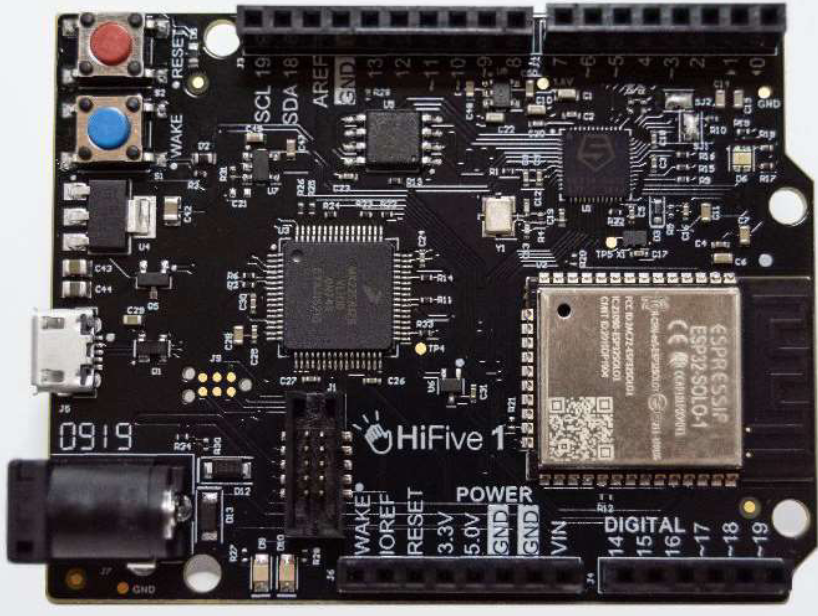
\includegraphics[width=0.6\columnwidth]{figures/board_image.png}
    \centering
    \caption[Sifive Hifive1 RevB]{This figure shows the Sifive Hifive1 RevB development board from the Hifive1 Rev B Schematics\cite{sifive_schematics}}
\end{figure}
This project will be done on the Sifive Hifive1 Rev B. This is the second iteration of the Hifive1 board, which uses the SiFive Freedom E310-G002 chip featuring a RV32IMAC core, a 16 KiB instruction cache, 16 KiB data RAM, and 32 MiB of Flash memory, which acts as ROM. It has Arduino compatible pins, a set of LEDs, a Bluetooth/WiFi chip, and a USB interface\cite{sifive_manual}.